\begin{table*}[!htp]
    \setlength{\tabcolsep}{4pt}
    % \footnotesize
    \floatconts
      {tab:table_ate_3_6}
      {\caption{Causal Inference ATE Estimates at Snapshots of 3 and 6 Months}\vspace{-.5em}}
      {\adjustbox{max width=.825\textwidth}{\begin{tabular}{l c c c c c }
    \toprule
    &T-learner & S-learner & Matching (1) & Matching (5) & Matching (20) \\
    \midrule
    \textit{(Snapshot: 3 months)} \\
    CoxPH & -3.524 ± 0.274 & -3.644 ± 0.393 & -4.245 ± 0.005 & -4.280 ± 0.003 & -4.406 ± 0.002 \\
    Random Survival Forest & -2.317 ± 0.602 & -1.183 ± 0.363 & -1.615 ± 0.073 & -1.538 ± 0.054 & -1.978 ± 0.050 \\
    DeepSurv & -2.366 ± 0.603 & -1.986 ± 0.382 & -2.160 ± 1.014 & -2.101 ± 1.051 & -2.312 ± 1.223 \\
    DeepHit & -2.956 ± 6.663 & 0.417 ± 0.967 & 0.215 ± 0.481 & 0.241 ± 0.476 & 0.200 ± 0.501 \\
    \midrule
    Causal Survival Forest &  \multicolumn{5}{c}{-3.045 ± 0.128 (Not a meta-learner method)}  \\
    \midrule \\
    \textit{(Snapshot: 6 months)} \\
    CoxPH & -2.910 ± 0.791 & -2.118 ± 0.751 & -2.578 ± 0.009 & -2.639 ± 0.006 & -2.900 ± 0.007 \\
    Random Survival Forest & -2.148 ± 0.957 & -0.925 ± 0.378 & -1.762 ± 0.191 & -1.569 ± 0.135 & -1.807 ± 0.109 \\
    DeepSurv & -3.685 ± 1.998 & -0.516 ± 1.284 & -1.877 ± 0.708 & -1.927 ± 0.594 & -2.152 ± 0.422 \\
    DeepHit & 11.551 ± 3.806 & -1.022 ± 0.428 & 0.007 ± 0.727 & 0.054 ± 0.804 & 0.140 ± 0.876 \\
    \midrule
    Causal Survival Forest &  \multicolumn{5}{c}{-2.831 ± 0.101 (Not a meta-learner method)}  \\
    \bottomrule
    \end{tabular}}\vspace{-1em}}
    % \footnotetext{Not a meta-learner method.}
\end{table*}


In this section, we present our findings on survival analysis prediction performance and on causal inference treatment effect estimates.
Performance metrics are computed at snapshots of \(\tau \in \{3, 6, 9, 12\}\) months.
The main body highlights results at 3 and 6 months, while detailed outcomes for 9 and 12 months are included in Appendix~\ref{apd:survival_analysis} and Appendix~\ref{apd:causal_inference}. 
A comparison of unadjusted survival curves is provided in Appendix~\ref{apd:unadjusted_survival}, demonstrating that the observed Average Treatment Effects (ATEs) cannot be fully attributed to baseline differences between groups.

For transparency and reproducibility\footnote{Code is available in at \url{https://github.com/Shahriarnz14/causal-meta-learner-survival-analysis}}, we provide details on data preprocessing, training protocols, and model hyperparameters in Appendices~\ref{apd:preprocessing} and~\ref{apd:model_hyperparams}.
Additionally, Appendix~\ref{apd:cohort_information} provides a comprehensive breakdown of the study cohort, including demographics, adverse events, adherence patterns, and prescribing trends, offering essential context on the patient population and factors influencing adherence. 

% \vspace{-1em}
\subsection{Results: Adverse Event Time Prediction}
\label{sec:04_results_survival}
% \vspace{-0.25em}

We begin by looking at the prediction performance of the survival models from Section~\ref{sec:methods_survival}.
Tables~\ref{tab:survival_3_6} and~\ref{tab:survival_9_12} report the time-dependent Concordance Index (\(C^{td}\)), Integrated Brier Score (IBS), and time-dependent Area Under the Curve (\(\text{AUC}^{td}\)) for each survival model--Cox proportional hazards (CoxPH), Random Survival Forest (RSF), DeepSurv, and DeepHit--across the four snapshot horizons. 

Across different prediction time snapshots, RSF consistently outperforms other models in terms of \(C^{td}\) and \(\text{AUC}^{td}\) while achieving lower IBS values, suggesting superior calibration and predictive reliability.
CoxPH and DeepSurv exhibit similar performance trends, with CoxPH maintaining slightly higher discriminative ability at later time points, whereas DeepSurv performs better at shorter horizons.

DeepHit underperforms across all time points, with lower \(C^{td}\) and \(\text{AUC}^{td}\) values and higher IBS scores, indicating weaker discrimination and calibration.
At 3 months, its \(C^{td}\) is 0.570 and \(\text{AUC}^{td}\) is 0.588, the lowest among all models, and this trend persists at later horizons, with \(C^{td}\) dropping to 0.540 by 12 months.

The superior performance of RSF suggests its strength in capturing nonlinear relationships and complex interactions among risk scores, demographic features, and adherence patterns.
In contrast, CoxPH is interpretable but limited by its linearity and proportional hazards assumptions, reducing its flexibility in capturing complex dependencies.
DeepSurv and DeepHit exhibit larger variability performance metrics, possibly due to hyperparameter sensitivity.

% \vspace{-1em}
\subsection{Results: ATE Estimation}
\label{sec:04_results_causal}
% \vspace{-0.25em}

Tables~\ref{tab:table_ate_3_6} and~\ref{tab:table_ate_9_12} present the Average Treatment Effect (ATE) estimates for non-adherence at 3, 6, 9, and 12 months\footnote{Appendix~\ref{adp:from_assoc_to_causal} outlines the assumptions required for causal interpretation of our results.}.
Negative ATE values indicate that non-adherence is associated with a shorter adverse event time (i.e., an earlier occurrence of an adverse event) compared to adherence.
Figure~\ref{fig:graphical_ATE_trend} shows the ATE trends for each method across time snapshots.

Several key observations emerge from the ATE estimates. 
At early time points (3, 6, and 9 months), most models indicate that non-adherence is associated with earlier adverse events, with ATE estimates generally ranging from -0.5 to -4 months. 
Matching-based estimators tend to yield the most negative estimates, reinforcing the association between non-adherence and a shorter time to adverse event. 
The Causal Survival Forest (CSF) provides relatively stable estimates, consistently showing a negative ATE.

DeepHit exhibits high variability in its ATE estimates, sometimes producing values that deviate significantly from those of other models. 
Notably, at 6 months, DeepHit reports an ATE of \(11.551 \pm 3.806\), far from the estimates given by other methods. 
This instability aligns with its poor performance in survival analysis, where it consistently showed the lowest \(C^{td}\) and \(\text{AUC}^{td}\) scores and the highest IBS values.

In contrast, Random Survival Forest (RSF) not only achieves strong predictive performance in survival analysis but also provides more stable ATE estimates, consistently reporting negative values across time points, aligning with broader trends observed in other models. 

The negative ATE estimates at early time points align with clinical expectations that sustained medication adherence can stabilize patients with severe mental illness, thereby reducing the risk of crisis events.
Additionally, robust models such as RSF and CoxPH produce relatively consistent ATE estimates across different causal estimation approaches, including T-learners, S-learners, and matching-based estimators.
This consistency further supports the reliability of these estimates.
However, despite adjustments using demographic variables and county-provided risk scores, residual time-varying confounding may still influence these estimates, suggesting a need for more advanced causal modeling approaches that explicitly account for dynamic adherence and confounding effects.

\begin{figure*}[!ht]
\floatconts
  {fig:ite_injectable}
  {\vspace{-2em} \caption{
  Distribution of Estimated Individual Treatment Effects (ITE) for different medication adherence groups: \textcolor{ForestGreen}{injectable}, \textcolor{orange}{non-injectable}, and \textcolor{purple}{not covered} at time snapshot \(\tau=3\) months. 
    Each plot's legend highlights the Average Treatment Effect (ATE) in months for the groups covered by \textcolor{ForestGreen}{injectable} medication, \textcolor{orange}{non-injectable} medication, and those \textcolor{purple}{not covered} by any medication. 
  (a)-(c): T-learner ITEs for CoxPH, DeepSurv, and Random Survival Forest. 
  (d): ITE for Causal Survival Forest.}\vspace{-1em}}
  {%
    \subfigure[\footnotesize (CoxPH, T-Learner)]{\label{fig:ite_injectable_coxph}%
      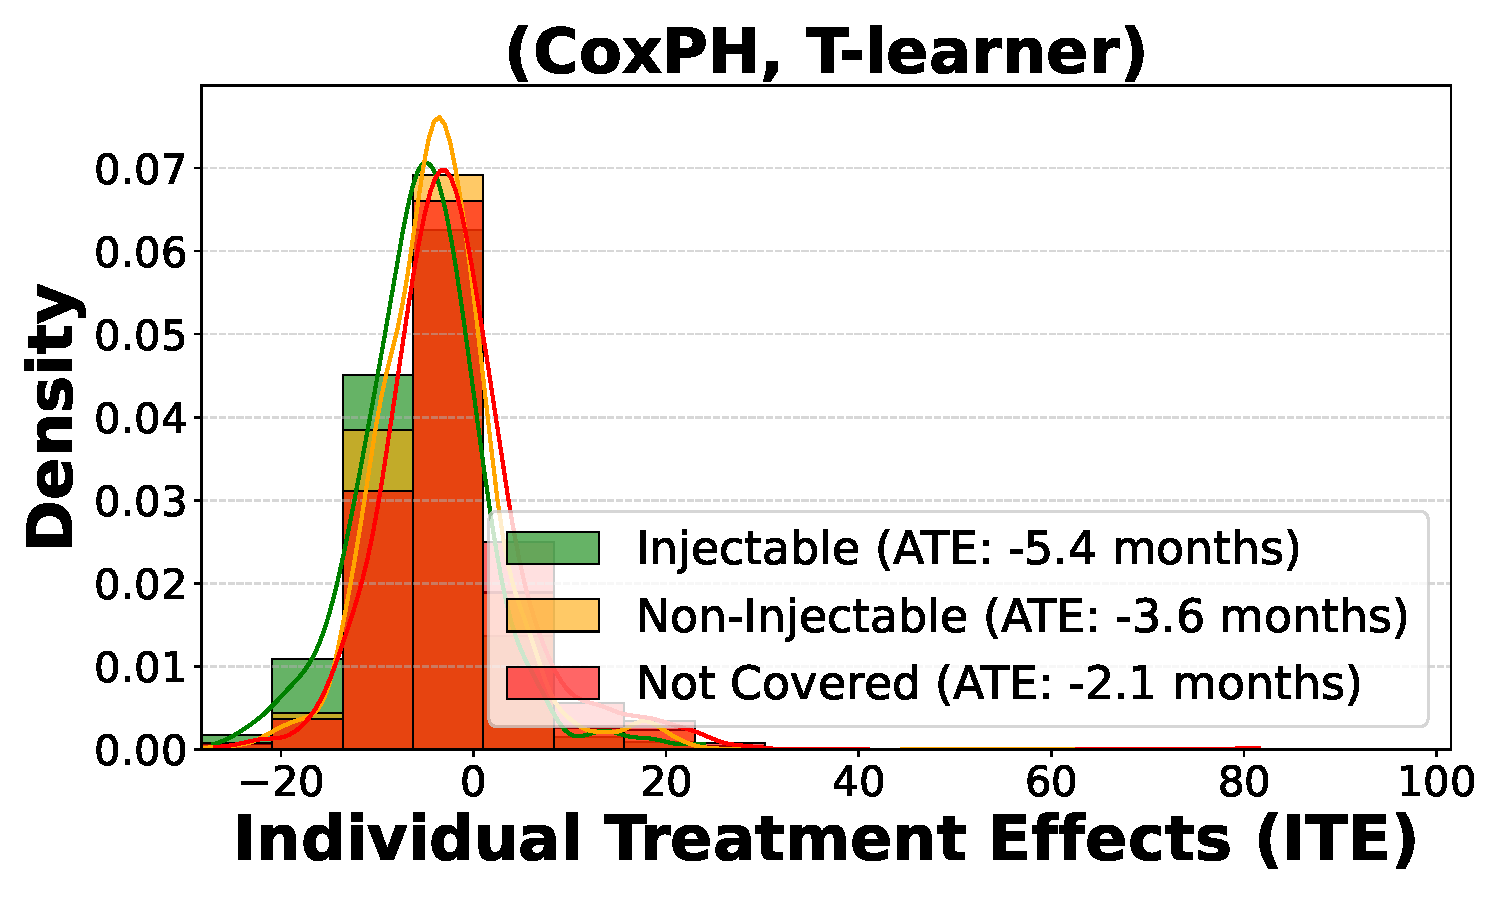
\includegraphics[width=.22\linewidth]{Figures/ITE_injectable/ITE_CoxPH_T-learner_injectable_type.pdf}}%
    \qquad
    \subfigure[\footnotesize (DeepSurv, T-Learner)]{\label{fig:ite_injectable_deepsurv}%
      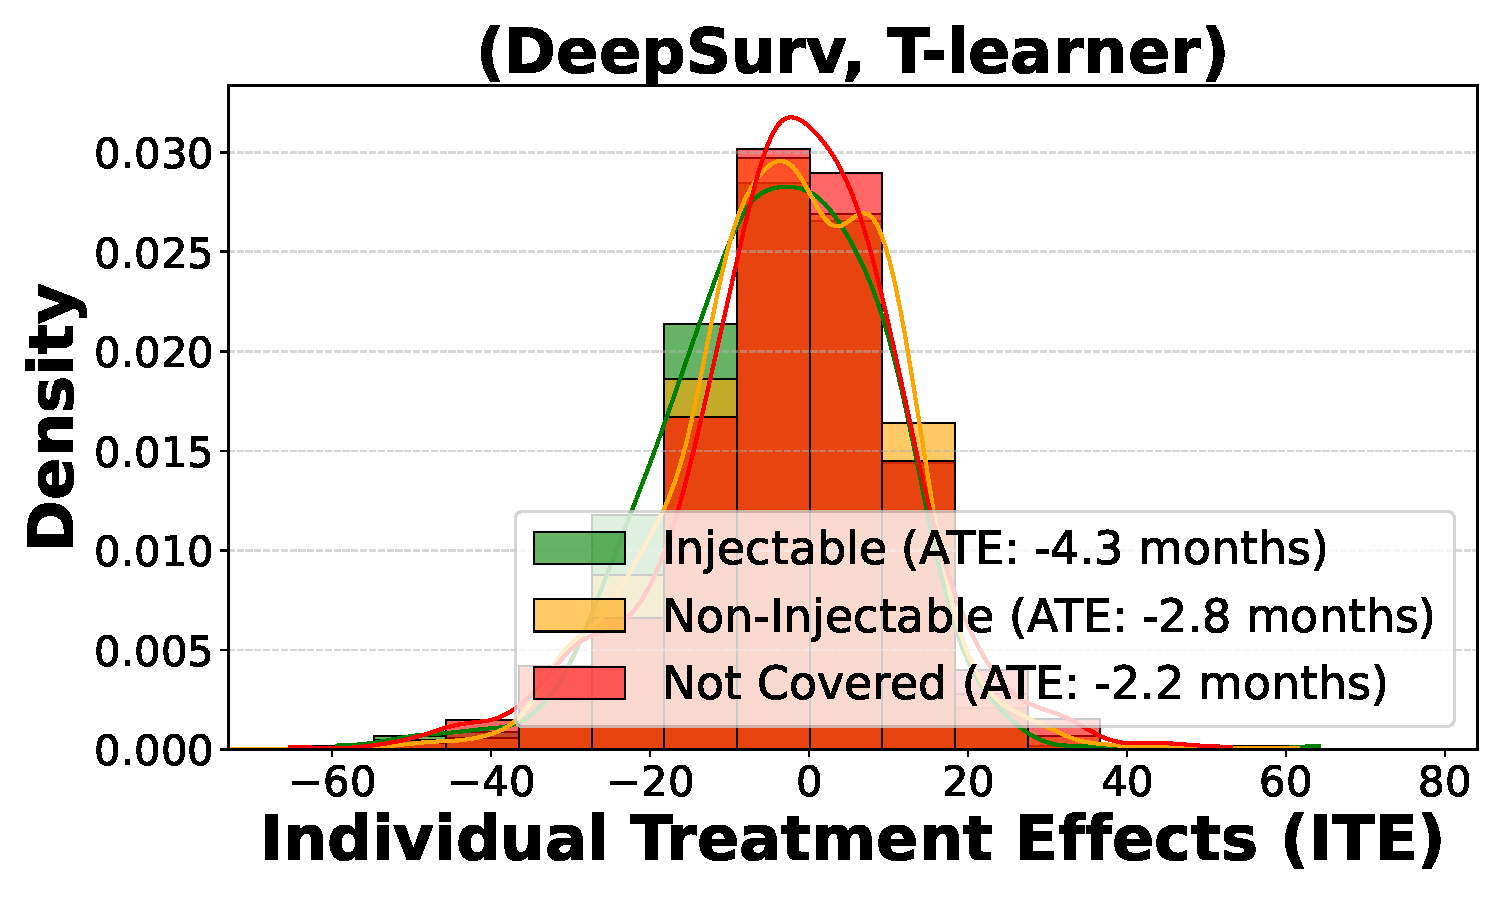
\includegraphics[width=.22\linewidth]{Figures/ITE_injectable/ITE_DeepSurv_T-learner_injectable_type.pdf}}%
    \qquad
    \subfigure[\footnotesize (RandomSurvivalForest, T-Learner)]{\label{fig:ite_injectable_random_survival_forest}%
      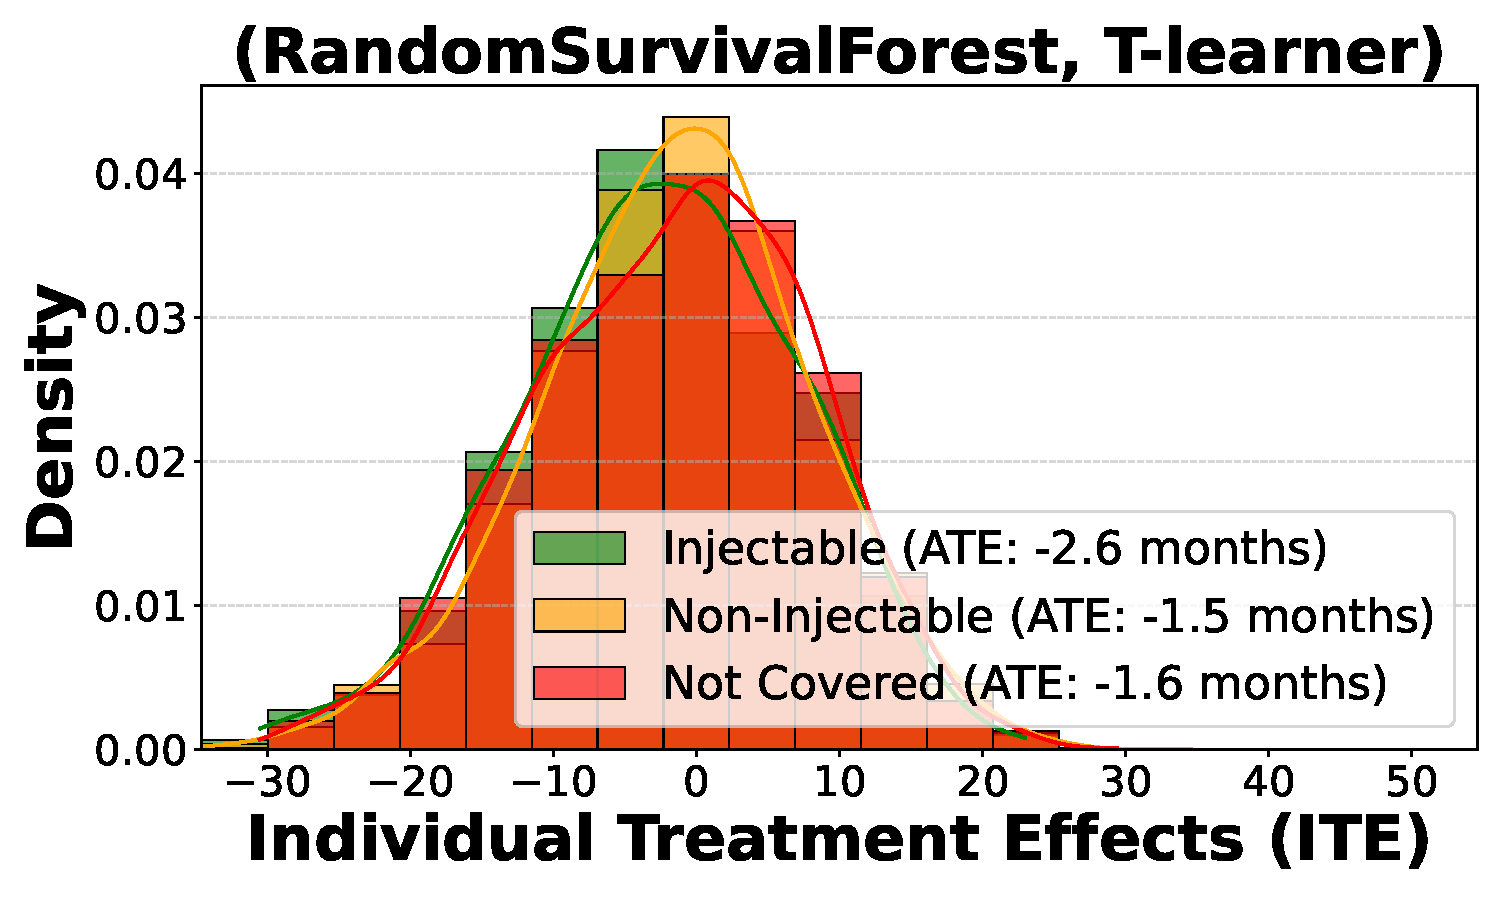
\includegraphics[width=.22\linewidth]{Figures/ITE_injectable/ITE_RandomSurvivalForest_T-learner_injectable_type.pdf}}%
    \qquad
    \subfigure[\footnotesize CausalSurvivalForest]{\label{fig:ite_injectable_causal_survival_forest}%
      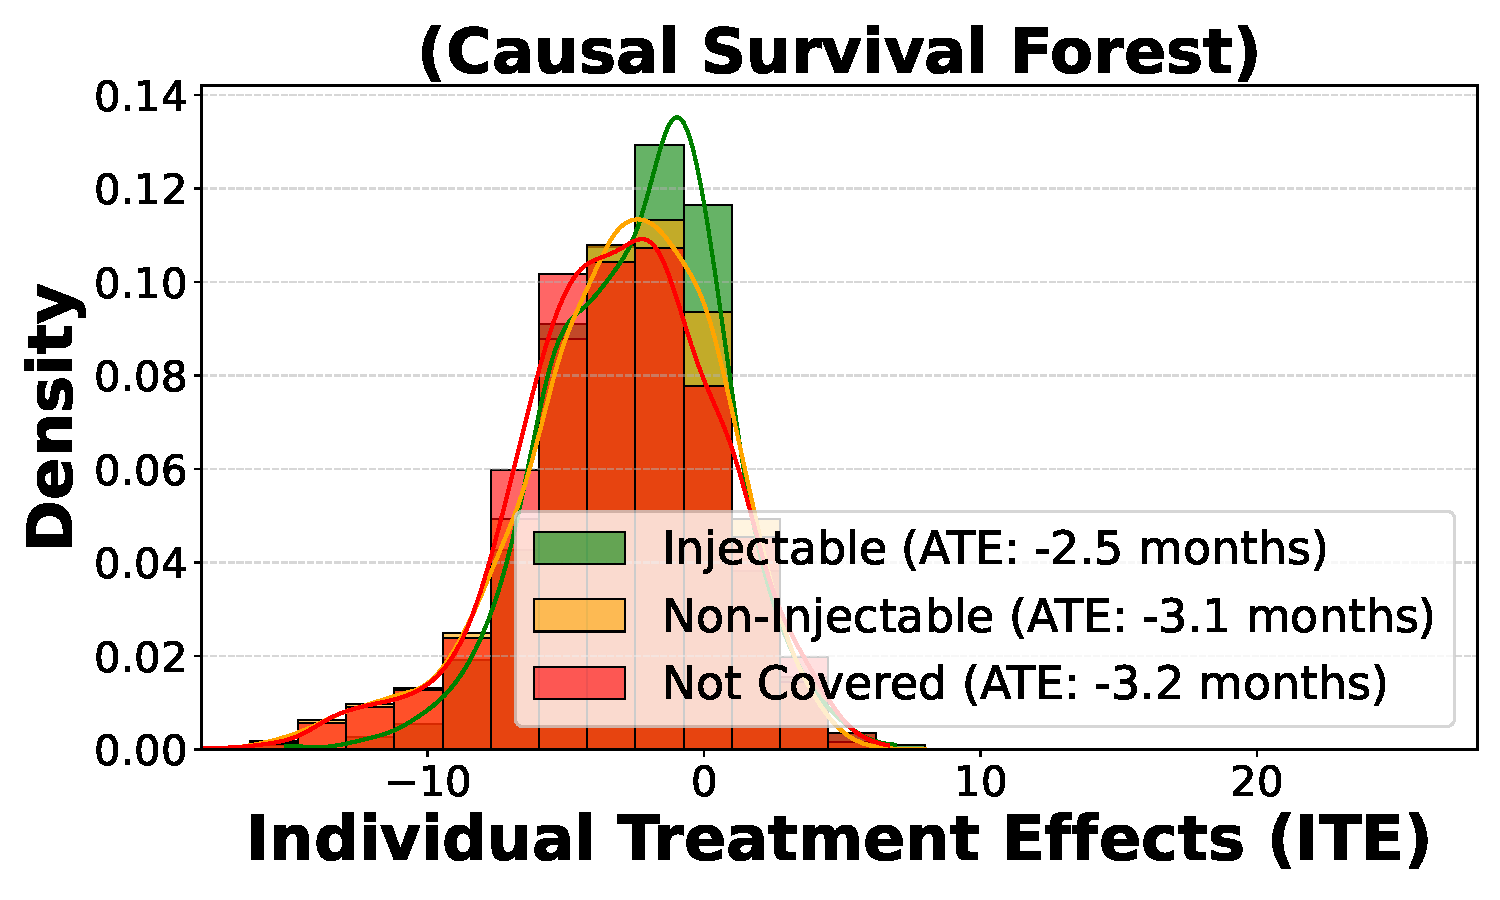
\includegraphics[width=.21\linewidth]{Figures/ITE_injectable/ITE_CausalSurvivalForest_Causal_Survival_Forest_injectable_type.pdf}}%
  }\vspace{-1.25em}
\end{figure*}

By 12 months, some ATE estimates, including those from RSF and CSF, shift toward zero or even become positive. 
For instance, CSF reports an ATE of \(0.345 \pm 0.097\), suggesting that adverse event time differences between adherent and non-adherent groups diminish at later snapshots. 
Rather than reflecting a genuine weakening of the treatment effect, this trend likely arises from selection dynamics, as each snapshot only includes individuals who have not had an adverse event up to that point, potentially biasing the estimates toward a ``healthier'' subset. 
Additionally, residual time-varying confounding may contribute to this shift if certain survival-influencing factors are not fully accounted for in the estimators.

% \vspace{-1.5em}
\subsection{Ablation Study: How ATE Estimates Change When Risk Scores are Removed}
\label{sec:04_results_ablation}
% \vspace{-0.25em}

We next examine the impact of removing the county-provided risk scores on the ATE estimates for different survival analysis model and causal inference method pairs. 
\cref{tab:table_ablation_CoxPH,tab:table_ablation_RandomSurvivalForest,tab:table_ablation_DeepSurv,tab:table_ablation_DeepHit,tab:table_ablation_RandomSurvivalForest} in Appendix~\ref{apd:ablation} compare the estimates obtained with the full model versus those from the ablated model (without risk scores) at the snapshot time 3, 6, 9, and 12 months. 
Notably, the magnitude of the negative ATE increases in the ablated models across all time horizons, suggesting that the risk scores partially capture confounding factors. 
Their removal amplifies the estimated impact of non-adherence, suggesting that these scores encode important latent risk factors that, when included, help account for confounding effects.

% \vspace{-1.5em}
\subsection{ITE Distribution for Different Medication}
\label{sec:04_results_ite_analysis}
% \vspace{-.5em}

We conducted a subgroup analysis to compare the distribution of Estimated Individual Treatment Effects (ITE) across three adherence groups: patients covered by injectable medications, non-injectable medications, and those not covered by any medication at the time snapshot \(\tau=3\) months.
Figure~\ref{fig:ite_injectable} presents the ITE distributions for each adherence group using various survival models and meta-learners.
The ITEs reflect the change in Restricted Mean Event Time (RMET) when comparing a non-adherence scenario to adherence within each category.

For the T-learner-based approaches using survival models, the ATEs for injectable medications appear slightly more negative compared to the non-injectable or not-covered groups.
This trend is observed in Figures~\ref{fig:ite_injectable_coxph}, \ref{fig:ite_injectable_deepsurv}, and \ref{fig:ite_injectable_random_survival_forest}, corresponding to CoxPH, DeepSurv, and Random Survival Forest, respectively.
However, the Causal Survival Forest results in Figure~\ref{fig:ite_injectable_causal_survival_forest} do not show a similar distinction, with ATEs for injectables being closer to the non-injectable and not-covered groups.

Overall, the ATEs across all survival models remain close within each formulation group, suggesting no meaningful differences in RMET across injectable, non-injectable, and not-covered groups in our dataset.
The ITE distributions also highlight some variability across models, with Random Survival Forest showing relatively narrower distributions compared to the other methods.
Further subgroup analysis is detailed in Appendix~\ref{apd:ite_injectable_all} for all models and meta-learners and follow the same pattern observed in Figure~\ref{fig:ite_injectable}.

These consistent negative ATE values align with the results reported in Section~\ref{sec:04_results_causal}, indicating shorter adverse event times associated with non-adherence across all adherence categories and medication types.
If nuanced differences existed in ITEs for injectable versus non-injectable formulations, they might have highlighted heterogeneity in treatment effects based on the delivery mechanism of medications.
However, the lack of such variation suggests that the adherence effect may be largely uniform across these groups in the context of our dataset.

In Section~\ref{apd:ite_medication}, we conducted a similar analysis for ITEs by medication type, observing close ATE values across the top four antipsychotic medications --risperidone, aripiprazole, olanzapine, and haloperidol-- with minimal differences in RMETs for non-adherence within each medication, showing no heterogeneity across medication type as well.

These findings indicate no significant heterogeneity in treatment effects across medication formulations or specific antipsychotic medications.
While slight variations in ATE rankings are observed across models, the magnitudes remain similar, suggesting that the adherence effect is largely stable regardless of medication type or delivery mechanism.